\chapter{GPU Convolution}
\label{chap:gpu_convolution}
Convolution is one of the most important tools in digital signal processing.
The PAQ system explained in Chapter \ref{sec:systemOverview} uses convolution at least 10 times, depending on the number of CMA iterations.
If convolution execution time improves by 10 ms, the full system execution time improves by 100 ms.
This chapter explores the how to optimize GPU convolution.

Discrete time convolution can be implemented in the time or frequency domain. 
Discrete time convolution computed in the time domain is
\begin{equation}
y(n) = \sum^{L-1}_{m=0} x(m) h(n-m)
  \label{eq:simple_conv_time}
\end{equation}
and discrete time convolution computed in the frequency domain is
\begin{equation}
\mathbf{y} = \mathscr{F}^{-1}(\mathscr{F}(\mathbf{x})\times\mathscr{F}(\mathbf{h}))
  \label{eq:simple_conv_freq}
\end{equation}
where the $N$ sample complex signal $\mathbf{x}$ is convolved with the $L$ tap filter complex $\mathbf{h}$.

Traditionally the number of flops is used to estimate how computationally intense an algorithm is. 
Each complex multiply 
\begin{equation}
(A+jB)\times(C+jD) = (AC-BD)+j(AD+BC)
\end{equation}
is $6$ flops, $4$ multiplies and $2$ additions/subtractions.
Each output element of $\mathbf{y}$ in Equation \eqref{eq:simple_conv_time} requires $8L$ flops.
Each term in the $L$ long summation takes $8$ flops, $6$ flops per multiply plus $2$ flops (real and imaginary)  for the sum.
The output vector $\mathbf{y}$ is $N+L-1$ samples long.
The number of flops required for convolution is
\begin{equation}
8L(N+L-1) \text{ flops}.
\label{eq:flops_time_domain_conv}
\end{equation}

The length of the convolution, $M=N+L-1$ is the minimum point Fourier Transform possible.
To leverage the Cooley-Tukey radix 2 Fast Fourier Transform (FFT), it is common practice append zeros to the next power of to above $M$.
The current most popular CPU based FFT is the Fastest Fourier Transform in the West (FFTW) library, FFTW uses the Cooley-Tukey radix 2 transform.
Each radix 2 forward or backward Fourier transform requires $5M\log_2(M)$ flops \cite{FFTW:2017,cooley1965algorithm}.
As shown by Equation \ref{eq:simple_conv_freq}, frequency domain convolution requires 
\begin{equation}
3\times5M\log_2(M)+6M \text{ flops}
\label{eq:flops_freq_domain_conv}
\end{equation}
from $3$ FFTs and a length $M$ point to point multiply.


Comparing Equations \ref{eq:flops_time_domain_conv} and \ref{eq:flops_freq_domain_conv}, if a signal or filter length is relatively long the frequency domain is the best choice.
What constitutes a ``long'' signal or filter?
When should convolution be done in the frequency domain rather than time domain?

Figure \ref{fig:Theory12672signal_flops} compares the number of flop required to convolve a $12672$ sample complex signal with a varied length tap complex filter.
According to the number of flops in the figure, frequency domain convolution requires less flops if the filter is longer $40$ taps.
\begin{figure}
	\caption{Comparison of number of floating point operations (flops) required to convolve a $12672$ sample complex signal with a varied length tap complex filter.}
	\centering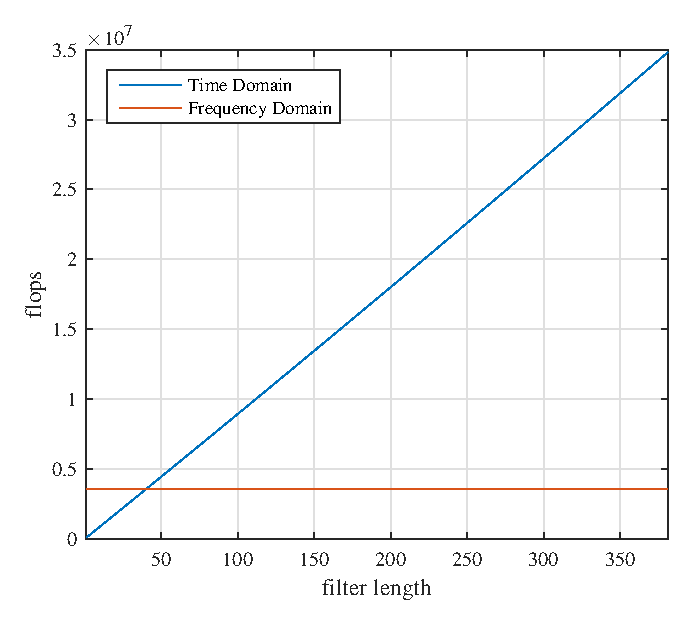
\includegraphics[width=5in]{figures/gpu_intro/Theory12672signal_flops.eps}
	\label{fig:Theory12672signal_flops}
\end{figure}

Figure \ref{fig:Theory186Tap_flops} compares the number of flops required for time domain verse frequency domain convolution of a $12672$ sample complex signal with a $186$ tap complex filter.
Figure \ref{fig:Theory21Tap_flops} compares the number of flops required for time domain verse frequency domain convolution of a $12672$ sample complex signal with a $21$ tap complex filter.
Appending zeros to the next power of $2$ causes the stair stepping pattern.
Judging by the figures with varied signal lengths, a $186$ tap filter is ``long'' and a $21$ tap filter is ``short.''
\begin{figure}
	\caption{Comparison of number of floating point operations (flops) required to convolve a varied length complex signal with a $186$ tap complex filter.}
	\centering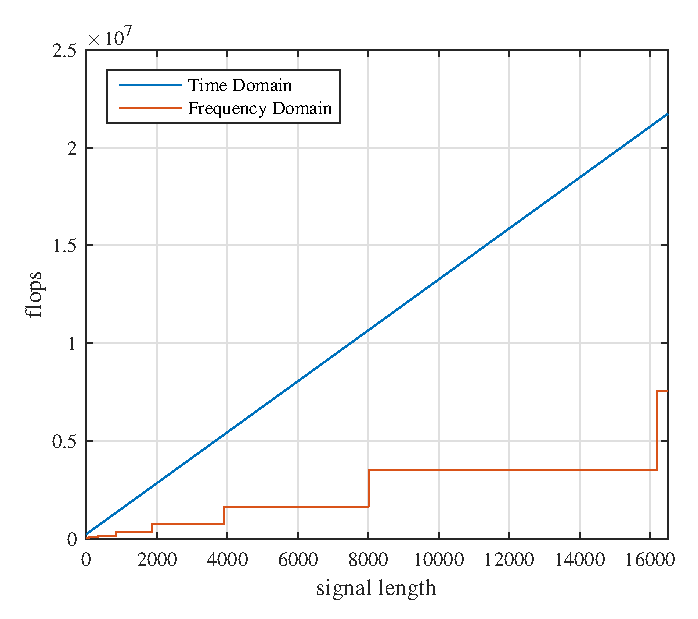
\includegraphics[width=5in]{figures/gpu_intro/Theory186Tap_flops.eps}
	\label{fig:Theory186Tap_flops}
\end{figure}
\begin{figure}
	\caption{Comparison of number of floating point operations (flops) required to convolve a varied length complex signal with a $21$ tap complex filter.}
	\centering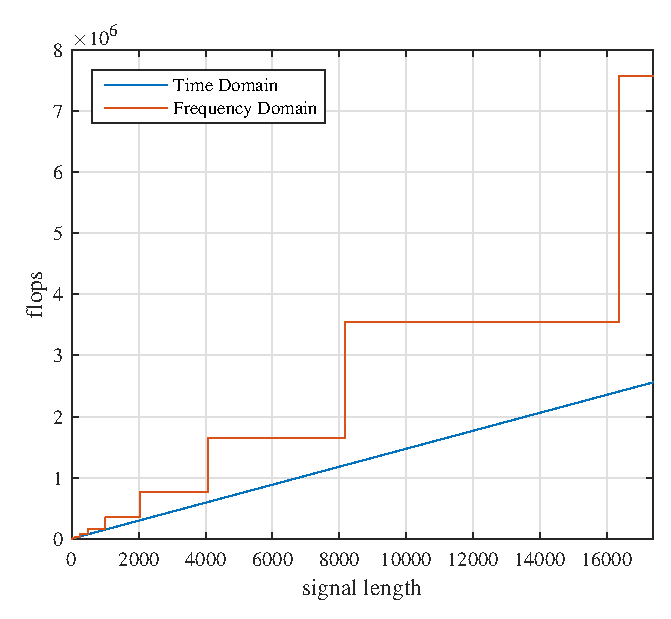
\includegraphics[width=5in]{figures/gpu_intro/Theory21Tap_flops.eps}
	\label{fig:Theory21Tap_flops}
\end{figure}



\section{CPU and GPU Single Batch Convolution}
\label{sec:cuda_convolution_single}
With an understanding of the number of flops in time verses frequency domain required to implement convolution,
do the number of flops have a direct relationship to execution time in CPUs and GPUS?
To explore the flop to execution time relationship Listing \ref{code:convFun} shows five different ways of implementing convolution:
\begin{itemize}
  \item time domain convolution in a CPU
  \item frequency domain convolution in a CPU
  \item time domain convolution in a GPU using global memory
  \item time domain convolution in a GPU using shared memory
  \item frequency domain convolution in a GPU using CUDA libraries
\end{itemize}

The CPU implements Equation \eqref{eq:simple_conv_time} in ConvCPU directly on line $209$ using a function from lines $11$ to $34$.
The CPU implements Equation \eqref{eq:simple_conv_freq} using the FFTW library on lines $214$ to $258$.

The GPU implements time domain convolution using global memory in lines $268$ to $277$.
The GPU kernel ConvGPU on lines $36$ to $64$ is a parallel version of ConvCPU.
ConvGPU performs time domain convolution by fetching every element of the signal and filter from global memory.

The GPU implements time domain convolution using shared memory in lines $283$ to $292$.
The GPU kernel ConvGPUshared on lines $67$ to $101$ is nearly identical to ConvGPU.
Threads accessing the same elements of the filter in global memory can be a waste of valuable clock cycles.
ConvGPUshared pays and initial price on lines $72$ to $76$ to move $L_\text{h}$ filter coefficients from off chip global memory to the on chip shared memory.
Finally, the GPU implements frequency domain convolution using the cuFFT library on lines $298$ to $326$.

The questions are:
Do flops have a direct relationship to execution time on CPUs? 
Do flops have a direct relationship to execution time on GPUs? 
When is the initial cost to use shared memory worth it?
When should convolution be done in the frequency domain?

The short answer to all of the questions is: GPU execution time depend on the signal length, filter length, CPU, GPU and memory.
A good CUDA programmer can make an educated guess on which algorithm may be faster in the GPU, but until all the algorithms have been implemented and timed, there is no definite answer.

To demonstrate that there is no definite answer in GPUs, 
the execution time of the code in Listing \ref{code:GPUvsCPU} was timed.
All the memory transfers to and from the host were timed for a fair comparison of GPU to CPU.
Table \ref{tab:CPUvsGPUtimingTable} shows where timing was started and stopped for each convolution implementation.
\begin{table}
\caption{Defining start and stop lines for timing comparison in Listing \ref{code:convFun}.}
\begin{center}
\begin{tabular}{llll}
	\toprule
	Algorithm 				& Function		& Start Line	& Stop  Line		\\ \midrule
	CPU time domain 		& ConvCPU 		& 208			& 210 				\\
	CPU frequency domain 	& FFTW 			& 213			& 259 				\\
	GPU time domain global 	& ConvGPU 		& 267			& 278				\\
	GPU time domain shared 	& ConvGPUshared & 282			& 293				\\
	GPU frequency domain 	& cuFFT			& 301			& 327				\\ 
	\bottomrule
\end{tabular}
\end{center}
\label{tab:CPUvsGPUtimingTable}
\end{table}

The execution times shown in Figure \ref{fig:CPUvsGPU_1batch_186taps_varySignal_noMin} compares the computation time of a fixed length $186$ tap filter convolved with a varied length signal.
The CPU execution time varies enough that the plot is messy.
Figure \ref{fig:CPUvsGPU_1batch_186taps_varySignal} shows the lower bounds of execution times by finding the local minimums in $15$ sample windows.
\begin{figure}
	\caption{Comparison of a complex convolution on CPU verse GPU. The signal length is varied and the filter is fixed at $186$ taps. The comparison is messy with out lower bounding.}
	\centering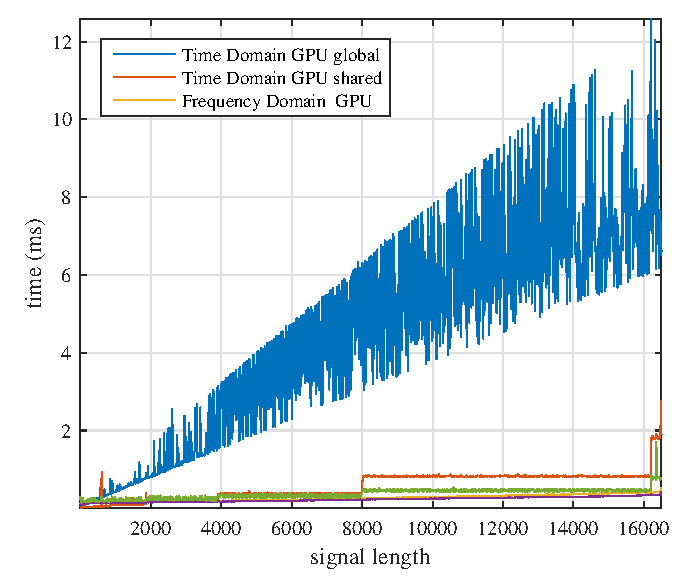
\includegraphics[width=5in]{figures/gpu_intro/CPUvsGPU_1batch_186taps_varySignal_noMin.eps}
	\label{fig:CPUvsGPU_1batch_186taps_varySignal_noMin}
\end{figure}
\begin{figure}
	\caption{Comparison of a complex convolution on CPU verse GPU. The signal length is varied and the filter is fixed at $186$ taps. A lower bound was applied by searching for a local minimums in $15$ sample width windows.}
	\centering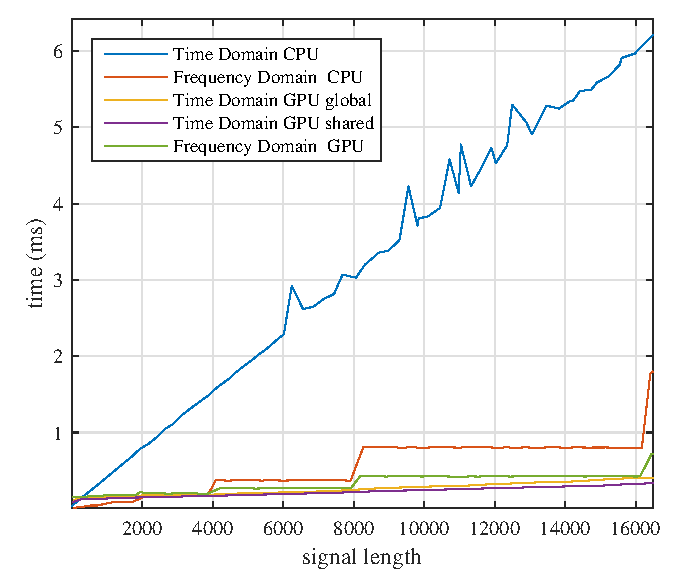
\includegraphics[width=5in]{figures/gpu_intro/CPUvsGPU_1batch_186taps_varySignal.eps}
	\label{fig:CPUvsGPU_1batch_186taps_varySignal}
\end{figure}

With the plot lower bounded, compare Figure \ref{fig:CPUvsGPU_1batch_186taps_varySignal} to Figure \ref{fig:Theory186Tap_flops}.
Does the CPU and GPU follow the same trend as the number of flops?
The CPU has the exact structure that the number of flops predicted.
The GPU does have the stair stepping from appending zeros for the frequency domain, but the time domain GPU kernels perform better than the number of flops predicted.

The GPU execution time does not follow the same trend as the number of flops.
Why? As mentioned in Section \ref{sec:GPU_memory}, GPUs have a ridiculous amount of computational resources and limited memory bandwidth.
Over $90\%$ of GPU kernels are memory bandwidth limited.
Fast GPU kernels access memory efficiently.

To provide more proof, compare Figures \ref{fig:CPUvsGPU_1batch_21taps_varySignal} and \ref{fig:Theory21Tap_flops}.
Once again, the CPU follows the same trend as the number of flops.
The GPU also follows the number of flops trends but to a lesser extent than the CPU.
Using shared memory will perform better than using only global memory for ``short'' filters.
\begin{figure}
	\caption{Comparison of a complex convolution on CPU verse GPU. The signal length is varied and the filter is fixed at $21$ taps. A lower bound was applied by searching for a local minimums in $5$ sample width windows.}
	\centering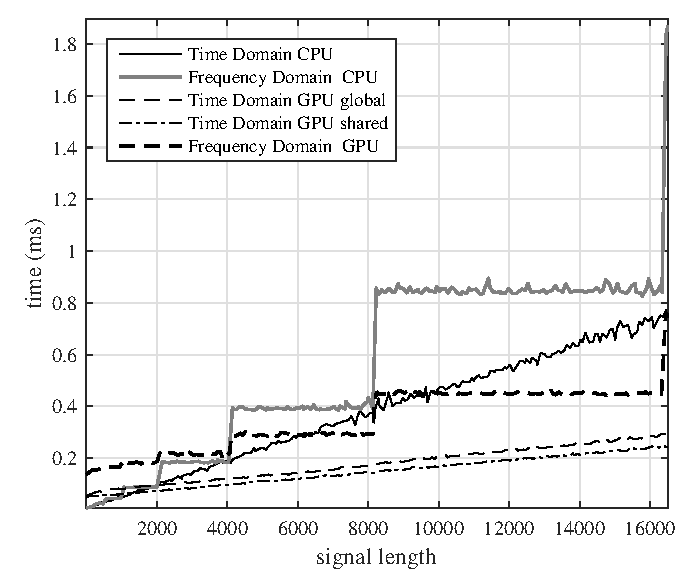
\includegraphics[width=5in]{figures/gpu_intro/CPUvsGPU_1batch_21taps_varySignal.eps}
	\label{fig:CPUvsGPU_1batch_21taps_varySignal}
\end{figure}

What if the signal length was set and the filter length was varied?
Comparing Figure \ref{fig:CPUvsGPU_1batch_12672signal_varyFilter} to Figure \ref{fig:Theory12672signal_flops} shows the CPU follows the trend of flops also.
The time domain CPU execution time is obviously affected as the number of flops increases.
Neither CPU or GPU frequency domain execution time is affected by varying filter length.

The execution time of both time domain GPU convolutions are slightly affected by increasing filter length.
The number of memory accesses per output sample increase as the filter length increases.
Bottom line, the length of the signal is the largest factor as Equations \ref{eq:flops_time_domain_conv} and \ref{eq:flops_freq_domain_conv} suggest.
\begin{figure}
	\caption{Comparison of a complex convolution on CPU verse GPU. The filter length is varied and the signal is fixed at $12672$ samples. A lower bound was applied by searching for a local minimums in $3$ sample width windows.}
	\centering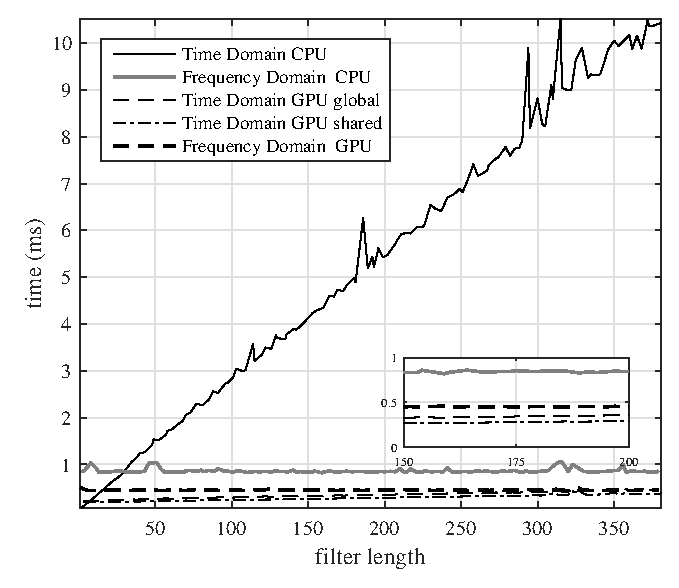
\includegraphics[width=5in]{figures/gpu_intro/CPUvsGPU_1batch_12672signal_varyFilter.eps}
	\label{fig:CPUvsGPU_1batch_12672signal_varyFilter}
\end{figure}

For most convolution implementations, the signal and filter lengths are set ``magic'' numbers.
To find the best option, implement convolution every way possible for the given lengths, time each implementation execution time, choose which algorithm is fastest.
As Figures \ref{fig:CPUvsGPU_1batch_186taps_varySignal_noMin} through \ref{fig:CPUvsGPU_1batch_12672signal_varyFilter} have shown, unless every implementation is explored, there is no way of saying which implementation will absolutely be fastest.

Table \ref{tab:CPUvsGPUtable_12672_186} shows the GPU frequency domain algorithm is fastest when convolving a $12672$ sample signal with a $186$ tap filter.
Table \ref{tab:CPUvsGPUtable_12672_21} shows the GPU time domain algorithm using shared memory is fastest when convolving a $12672$ sample signal with a $21$ tap filter.
\begin{table}
\caption{Convolution computation times with signal length $12672$ and filter length $186$ on a Tesla K40c GPU.}
\begin{center}
\begin{tabular}{lll}
	\toprule
	Algorithm 				& Function or Library		& Execution Time (ms) \\ \midrule
	CPU time domain 		& ConvCPU 					& 5.3000		\\
	CPU frequency domain 	& FFTW 						& 0.7972		\\
	GPU time domain global 	& ConvGPU 					& 0.3321		\\
	GPU time domain shared 	& ConvGPUshared 			& 0.2748		\\
	GPU frequency domain 	& cuFFT						& 0.4224		\\ 
	\bottomrule
\end{tabular}
\end{center}
\label{tab:CPUvsGPUtable_12672_186}
\end{table}
\begin{table}
\caption{Convolution computation times with signal length $12672$ and filter length $21$ on a Tesla K40c GPU.}
\begin{center}
\begin{tabular}{lll}
	\toprule
	Algorithm 				& Function or Library		& Execution Time (ms) \\ \midrule
	CPU time domain 		& ConvCPU 					& 0.5878		\\
	CPU frequency domain 	& FFTW 						& 0.8417		\\
	GPU time domain global 	& ConvGPU 					& 0.4476		\\
	GPU time domain shared 	& ConvGPUshared 			& 0.1971		\\
	GPU frequency domain 	& cuFFT						& 0.3360		\\ 
	\bottomrule
\end{tabular}
\end{center}
\label{tab:CPUvsGPUtable_12672_21}
\end{table}

\section{Batched Convolution}
As shown in section \ref{sec:cuda_convolution_single}, single convolution doesn't leverage the full power of parallel processing in GPUs.
Chapter \ref{sec:systemOverview} shows the PAQ received signal has a packetized structure.
The received signal has $3104$ packets or batches.
Batched processing introduces an extra level of parallelism in GPUs because each batch can be processed independently.
CUDA has many libraries that are ``batched,'' meaning a GPU kernel is launched for each independent packet or batch of received samples.
Some CUDA batched libraries used in PAQ system are cuFFT, cuBLAS and cuSolver.
%Figure \ref{fig:matrix_batch_vs_batched} shows the concept of a batched matrix multiply.
%\begin{figure}
%	\caption{Diagram showing the relationships between $z(n)$, $\rho(n)$ and $b(n)$.}
%	\centering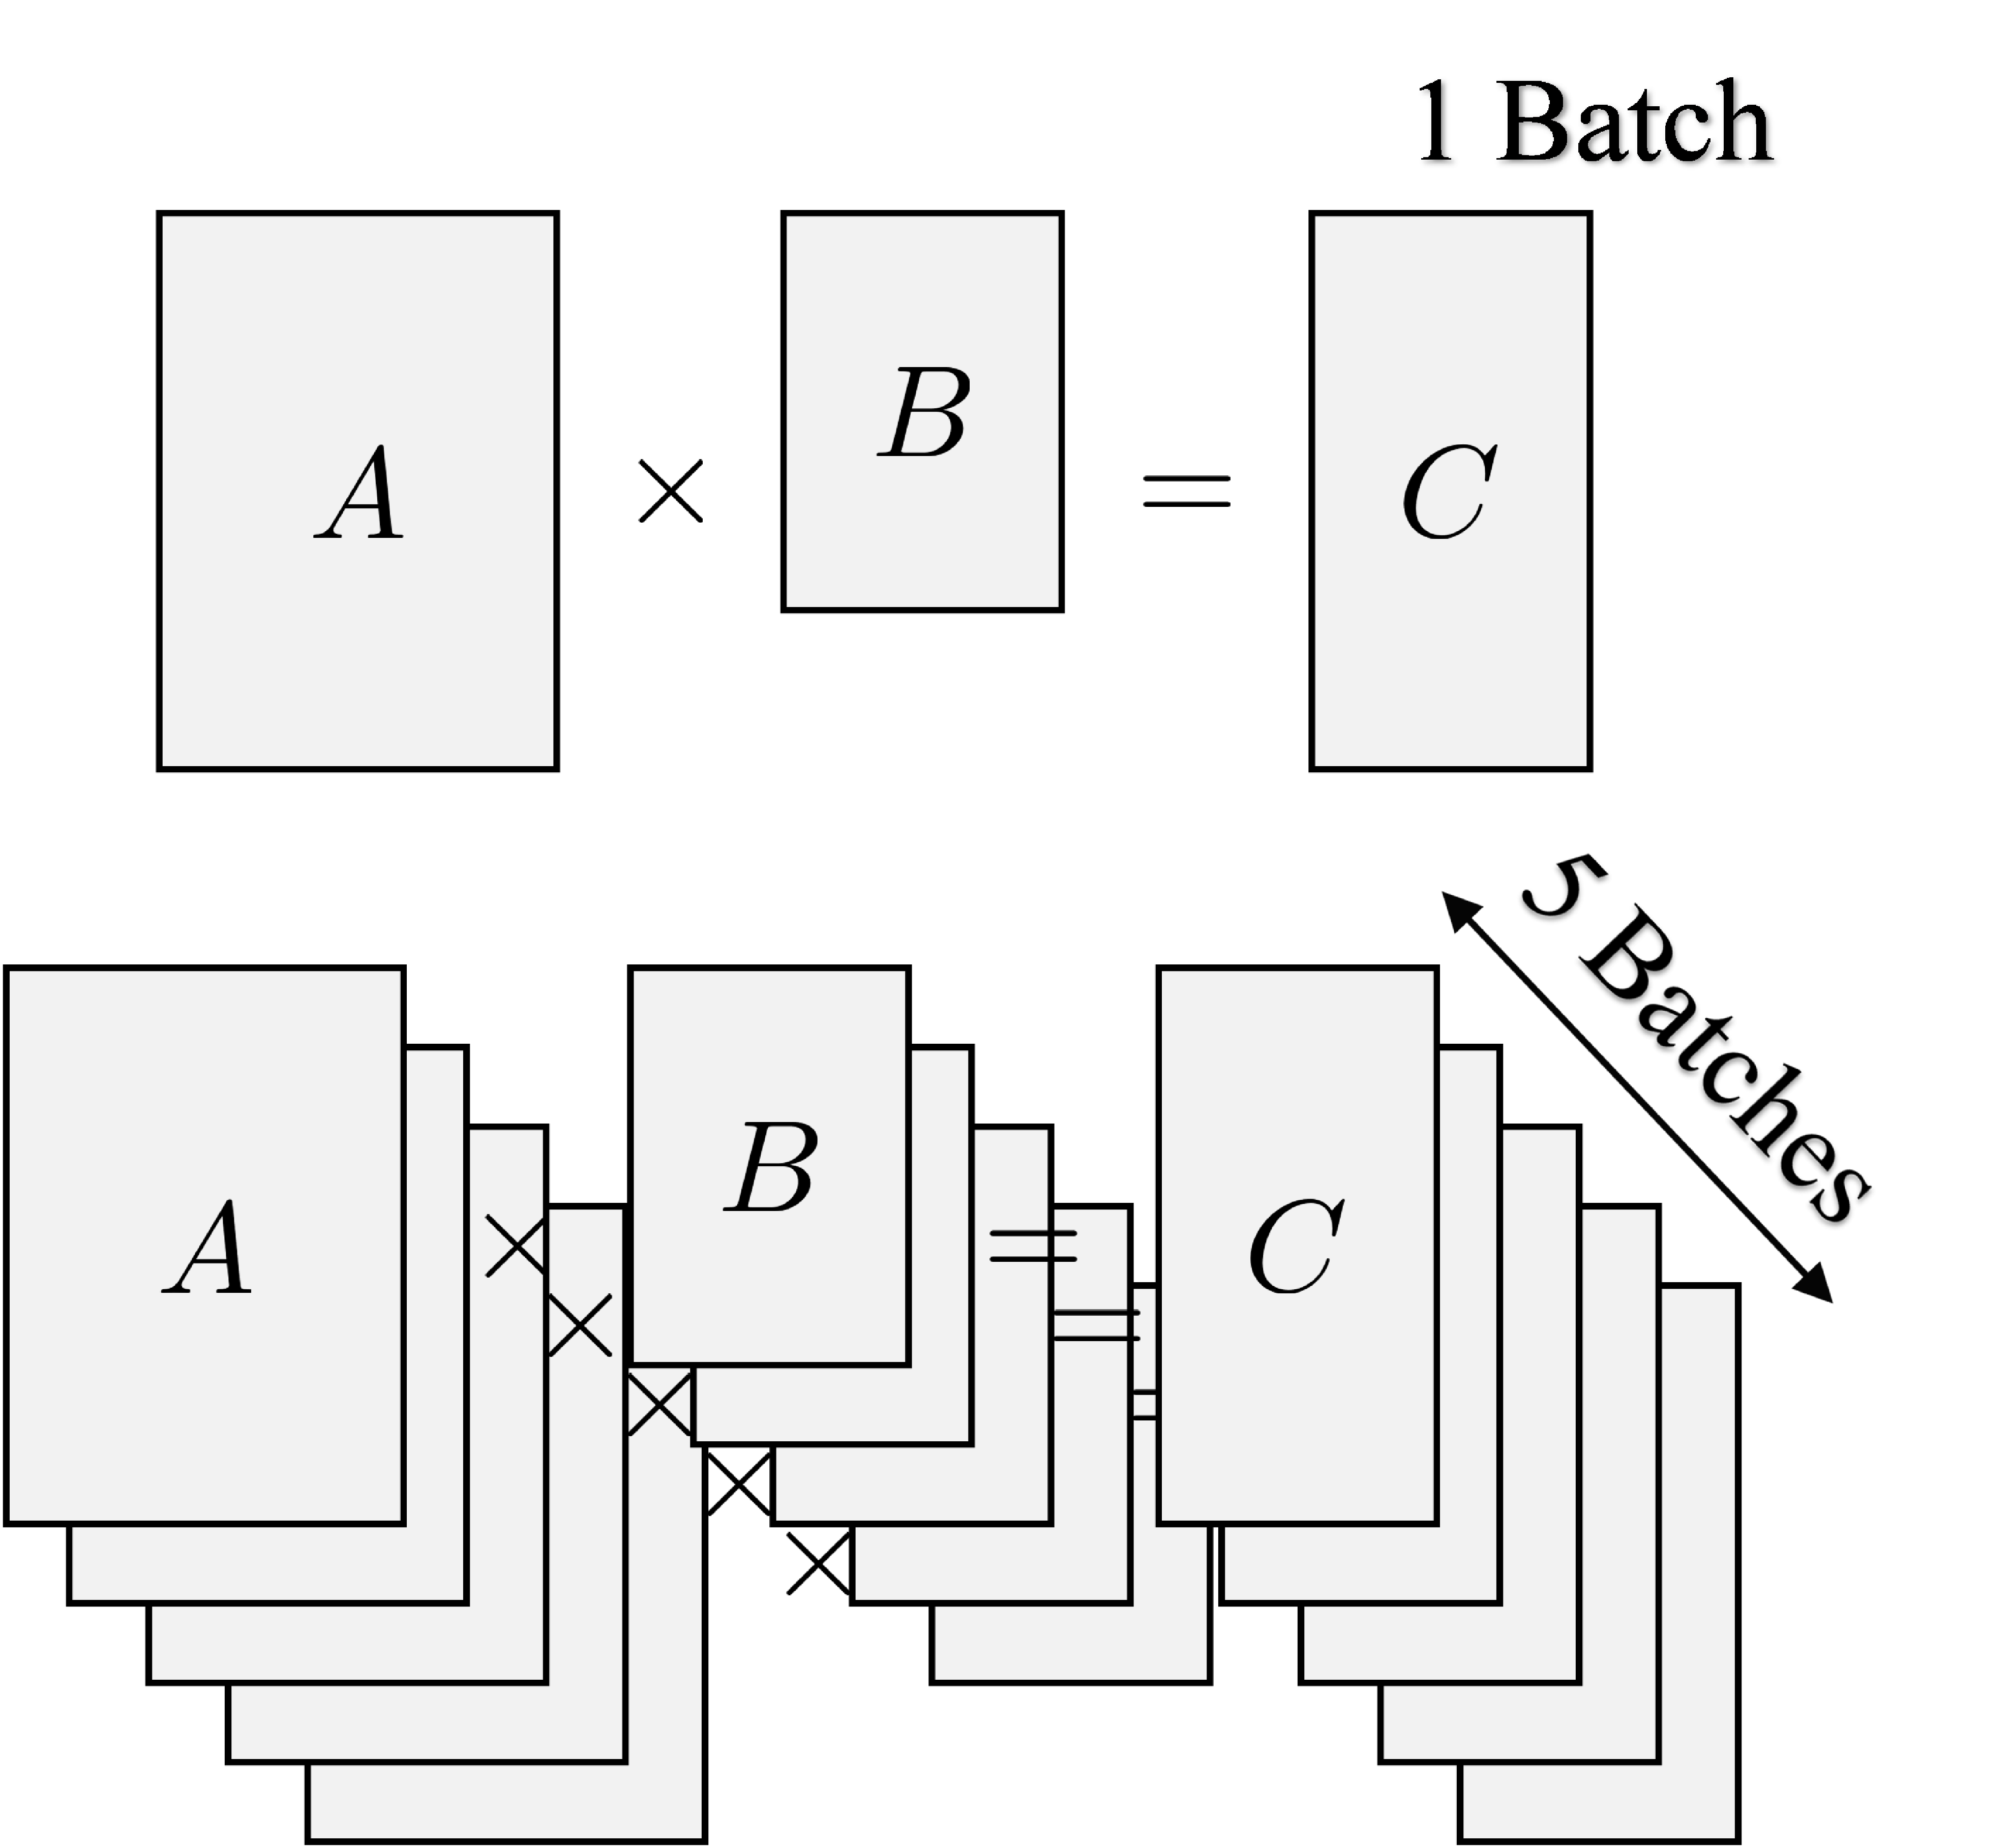
\includegraphics[width=4.13in/100*55]{figures/eq_GPUimplementation/matrix_batch_vs_batched.pdf}
%	\label{fig:matrix_batch_vs_batched}
%\end{figure}

Batched libraries perform much better than calling a single GPU kernel multiple times with each independent batch of data.
Haidar et al. showed batched libaries in GPUs achive more Gflops than calling GPU kernels multiple times \cite{haidar2015optimization}.
Batched processing performs very well in GPUs because it increases parallelism, reduces overhead on the CPU and provides more opportunities for NVIDIA engineers to optimize.

As the number of batches increases, does CPU and GPU execution time increase linearly?
To illistrate how batch processing performs on GPUs, Figure \ref{fig:CPUvsGPU_varyBatches_186taps_12672signal_timePerBatch} shows the execution time per batch for batched convolution in GPUs.
The execution time per batch decreases as the number of batches increases but converges after $70$ batches.
\begin{figure}
	\caption{Comparison on execution time per batch for complex convolution. The number of batches is varied while the signal and filter length is set to $12672$ and $186$.}
	\centering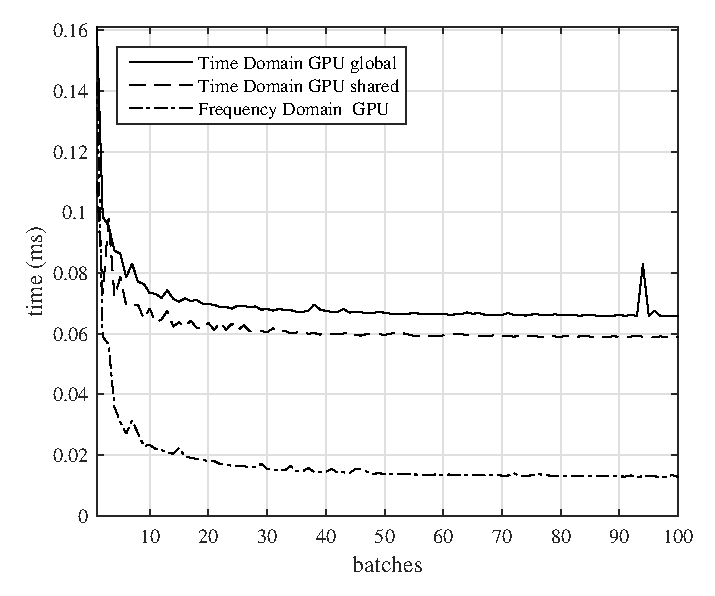
\includegraphics[width=5in]{figures/gpu_intro/CPUvsGPU_varyBatches_186taps_12672signal_timePerBatch.eps}
	\label{fig:CPUvsGPU_varyBatches_186taps_12672signal_timePerBatch}
\end{figure}

Figure \ref{fig:CPUvsGPU_varyBatches_186taps_12672signal} shows how the execution time increases with the number of batches varied.
Note that no lower bounding is needed to produce clean batched processing results.
This figure shows that frequency domain convolution leverages batch processing better than time domain convolution.
No surprise CPU time and frequency domain execution time skyrockets as the number of batches increases.
\begin{figure}
	\caption{Comparison of a batched complex convolution on a CPU and GPU. The number of batches is varied while the signal and filter length is set to $12672$ and $186$.}
	\centering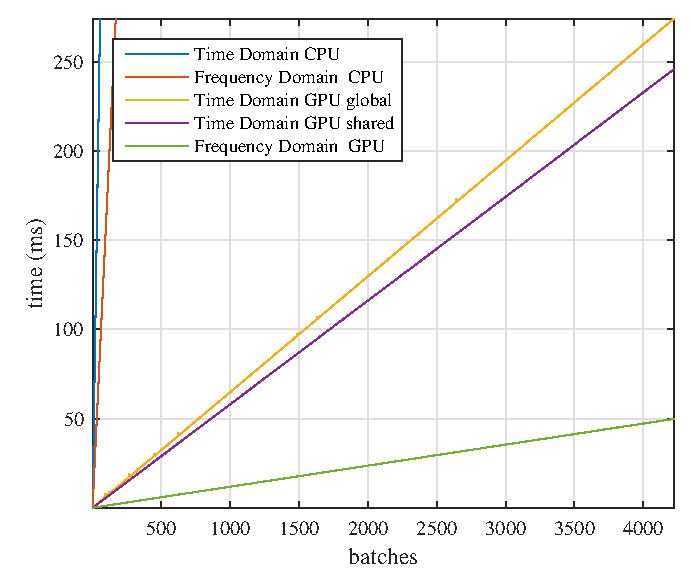
\includegraphics[width=5in]{figures/gpu_intro/CPUvsGPU_varyBatches_186taps_12672signal.eps}
	\label{fig:CPUvsGPU_varyBatches_186taps_12672signal}
\end{figure}

Judging by Figure \ref{fig:CPUvsGPU_varyBatches_186taps_12672signal}, CPU is not a contender in batched processing compared to the GPU.
CPU batched processing will not be explored any further.
Listing \ref{code:batchedConvFun} shows three implementations of batched convolution in CUDA
\begin{itemize}
  \item time domain convolution in a GPU using global memory
  \item time domain convolution in a GPU using shared memory
  \item frequency domain convolution in a GPU using the cuFFT library.
\end{itemize}

Now that the GPU execution time isn't being compared to the CPU, transfers between host and device will not be a factor for algorithm comparison.
Table \ref{tab:BatchedGPUtimingTable} shows how Listing \ref{code:batchedConvFun} is timed.
\begin{table}
\caption{Defining start and stop lines for timing comparison in Listing \ref{code:batchedConvFun}.}
\begin{center}
\begin{tabular}{llll}
	\toprule
	Algorithm 				& Function		& Start Line	& Stop  Line		\\ \midrule
	GPU time domain global 	& ConvGPU 		& 197			& 204				\\
	GPU time domain shared 	& ConvGPUshared & 212			& 219				\\
	GPU frequency domain 	& cuFFT			& 227			& 245				\\ 
	\bottomrule
\end{tabular}
\end{center}
\label{tab:BatchedGPUtimingTable}
\end{table}
Figure \ref{fig:CPUvsGPU_3104batch_186taps_varySignal} shows execution time for $3104$ batches of $186$ tap filters convolved with varying signal lengths.
Performing frequency domain convolution is always faster than time domain convolution because the cuFFT library is better optimized for batched processing.
The batched GPU implementation of convolution in the Frequency domain convolution takes just $36.8$ms for $3104$ batches, $12672$ sample signals and $186$ tap filters.
The average exectution time per batch for $3104$ batches is $0.0119$ms per batch!
Compare $0.0119$ms per batch to single batched execution time in Table \ref{tab:CPUvsGPUtable_12672_186}, one batch took $0.4224$.
Batched processing introduced a $35\times$ speed up!
\begin{figure}
	\caption{Comparison of a batched complex convolution on a GPU. The signal length is varied and the filter is fixed at $186$ taps.}
	\centering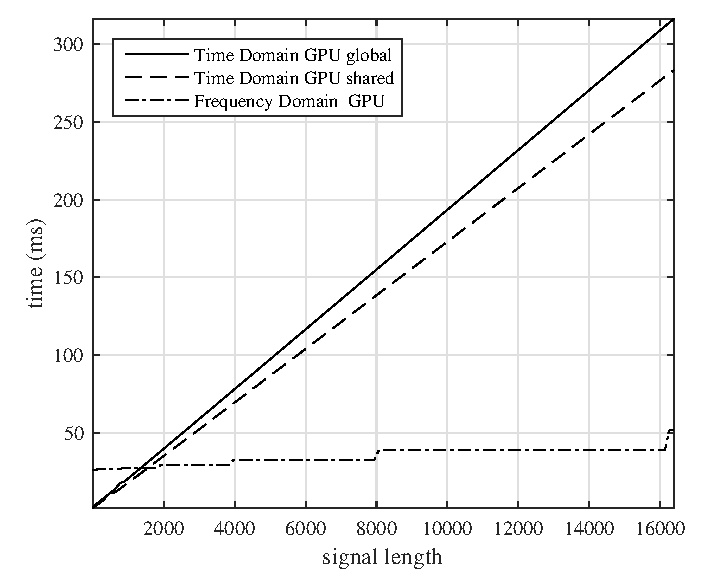
\includegraphics[width=5in]{figures/gpu_intro/CPUvsGPU_3104batch_186taps_varySignal.eps}
	\label{fig:CPUvsGPU_3104batch_186taps_varySignal}
\end{figure}

Figure \ref{fig:CPUvsGPU_3104batch_21taps_varySignal} shows execution time for $3104$ batches of $21$ tap filters convolved with varying signal lengths.
This figure exhibits the same characteristics of single batch convolution execution time shown in Figure \ref{fig:CPUvsGPU_1batch_21taps_varySignal}.
For most signal lengths, performing time domain convolution using shared memory is fastest.
\begin{figure}
	\caption{Comparison of a batched complex convolution on a GPU. The signal length is varied and the filter is fixed at $21$ taps.}
	\centering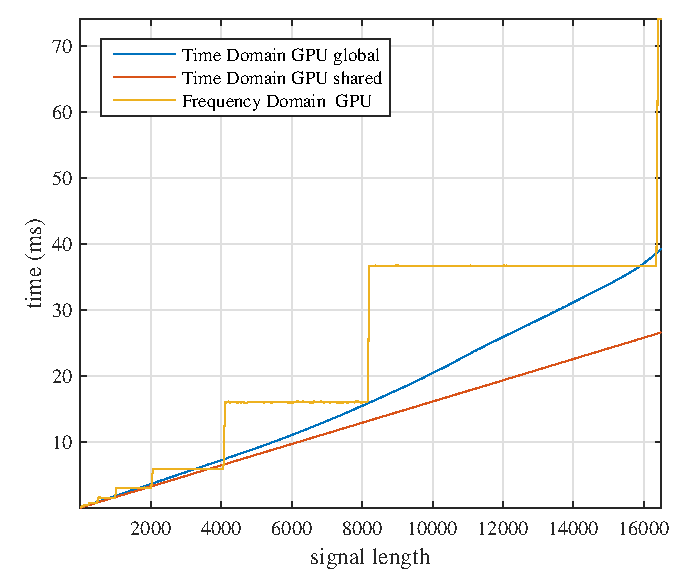
\includegraphics[width=5in]{figures/gpu_intro/CPUvsGPU_3104batch_21taps_varySignal.eps}
	\label{fig:CPUvsGPU_3104batch_21taps_varySignal}
\end{figure}

Figure \ref{fig:CPUvsGPU_3104batch_12672signal_varyFilter} shows execution time for $3104$ batches of $12672$ sample signal convolved with varying filter lengths.
This figure exhibits nearly the same characteristics of single batch convolution execution time shown in Figure \ref{fig:CPUvsGPU_1batch_12672signal_varyFilter} accept the varied filter length has no affect on execution time.
For very short filter lengths, time domain convolution using shared memory is fastest.
For longer filters , frequency domain convolution is fastest.
\begin{figure}
	\caption{Comparison of a batched complex convolution on a GPU. The filter length is varied and the signal length is set at $12672$ samples.}
	\centering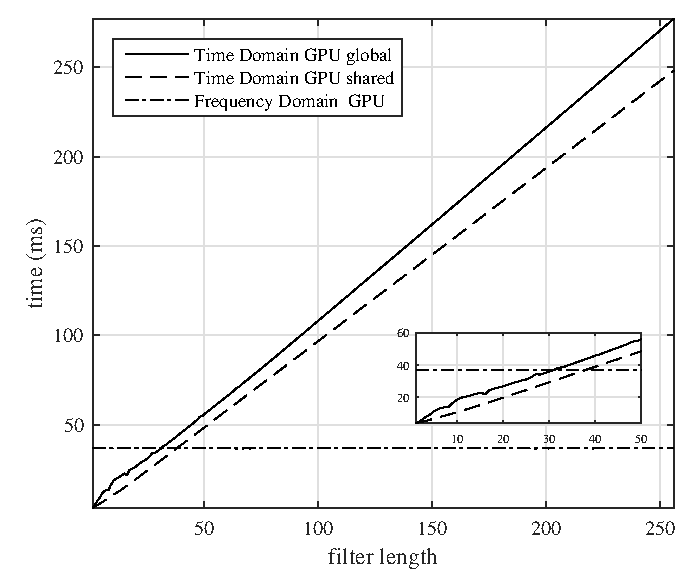
\includegraphics[width=5in]{figures/gpu_intro/CPUvsGPU_3104batch_12672signal_varyFilter.eps}
	\label{fig:CPUvsGPU_3104batch_12672signal_varyFilter}
\end{figure}

Though this section has show the power of batched processing, the algorithm leading to the fastest execution time still depends on signal and filter length,
One important concept has been over looked.
Figure \ref{fig:ProcessingBlock} shows there are two filters that need to be applied to the received samples. 

If convolution is implemented in the time domain, ConvGPU or ConvGPUshared must run twice.
The first call of time domain convolution performs an extremely fast ``short'' convolution of the $186$ tap equalizer and $21$ detection filter.
The second call performs a slower ``long'' convolution of the $12672$ sample signal with the  convolved $186+21-1$ tap filter.

If convolution is implemented in the frequency domain, only the GPU kernel PointToPointMultiply has to be updated.
PointToPointMultiply is changed from two to three input vectors.
For every point the number of memory accesses increases by $1$ element and the number of flops doubles from $6$ to $12$.
An extra cuFFT call would be expected accept the detection filter is predefined in Figure \ref{fig:ProcessingBlock}.
The FFT of the detection filter is calculated and stored at initialization.

Table \ref{tab:Batched_CPUvsGPUtable_12672_186} shows the batched convolution execution time for a $12672$ sample signal and $186$ tap filter.
Table \ref{tab:Batched_CPUvsGPUtable_12672_21} shows the batched convolution execution time for a $12672$ sample signal and $21$ tap filter.
Table \ref{tab:Batched_CPUvsGPUtable_12672_21_186} shows batched cascaded $21$ and $186$ tap filters convolved with a $12672$ sample signal execution time.
\begin{table}
\caption{Batched convolution execution times with for a $12672$ sample signal and $186$ tap filter on a Tesla K40c GPU.}
\begin{center}
\begin{tabular}{lll}
	\toprule
	Algorithm 				& Function or Library		& Execution Time (ms) \\ \midrule
	GPU time domain global 	& ConvGPU 					& 201.29		\\
	GPU time domain shared 	& ConvGPUshared 			& 180.272		\\
	GPU frequency domain 	& cuFFT						& 36.798 		\\ 
	\bottomrule
\end{tabular}
\end{center}
\label{tab:Batched_CPUvsGPUtable_12672_186}
\end{table}
\begin{table}
\caption{Batched convolution execution times with for a $12672$ sample signal and $21$ tap filter on a Tesla K40c GPU.}
\begin{center}
\begin{tabular}{lll}
	\toprule
	Algorithm 				& Function or Library		& Execution Time (ms) \\ \midrule
	GPU time domain global 	& ConvGPU 					& 27.642		\\
	GPU time domain shared 	& ConvGPUshared 			& 20.4287		\\
	GPU frequency domain 	& cuFFT						& 36.7604		\\ 
	\bottomrule
\end{tabular}
\end{center}
\label{tab:Batched_CPUvsGPUtable_12672_21}
\end{table}
\begin{table}
\caption{Batched convolution execution times with for a $12672$ sample signal and cascaded $21$ and $186$ tap filter on a Tesla K40c GPU.}
\begin{center}
\begin{tabular}{lll}
	\toprule
	Algorithm 				& Function or Library		& Execution Time (ms) \\ \midrule
	GPU time domain global 	& ConvGPU 					& 223.307		\\
	GPU time domain shared 	& ConvGPUshared 			& 200.018		\\
	GPU frequency domain 	& cuFFT						& 39.0769		\\ 
	\bottomrule
\end{tabular}
\end{center}
\label{tab:Batched_CPUvsGPUtable_12672_21_186}
\end{table}
\begin{table}
\caption{Batched convolution execution times with for a $12672$ sample signal and $206$ tap filter on a Tesla K40c GPU.}
\begin{center}
\begin{tabular}{lll}
	\toprule
	Algorithm 				& Function or Library		& Execution Time (ms) \\ \midrule
	GPU time domain global 	& ConvGPU 					& 223.064		\\
	GPU time domain shared 	& ConvGPUshared 			& 199.844		\\
	GPU frequency domain 	& cuFFT						& 36.7704		\\ 
	\bottomrule
\end{tabular}
\end{center}
\label{tab:Batched_CPUvsGPUtable_12672_206}
\end{table}

Tables \ref{tab:Batched_CPUvsGPUtable_12672_186} and \ref{tab:Batched_CPUvsGPUtable_12672_21} agree with Figures \ref{fig:CPUvsGPU_3104batch_21taps_varySignal} and \ref{fig:CPUvsGPU_3104batch_186taps_varySignal}.
Time domain convolution is faster with a short $21$ tap filter but frequency domain convolution is faster with a long $186$ tap filter.

\begin{figure}
	\caption{Two ways to convolve the signal $\mathbf{r}$ with the $186$ tap filter $\mathbf{c}$ and $21$ tap filter $\mathbf{d}$.}
	\centering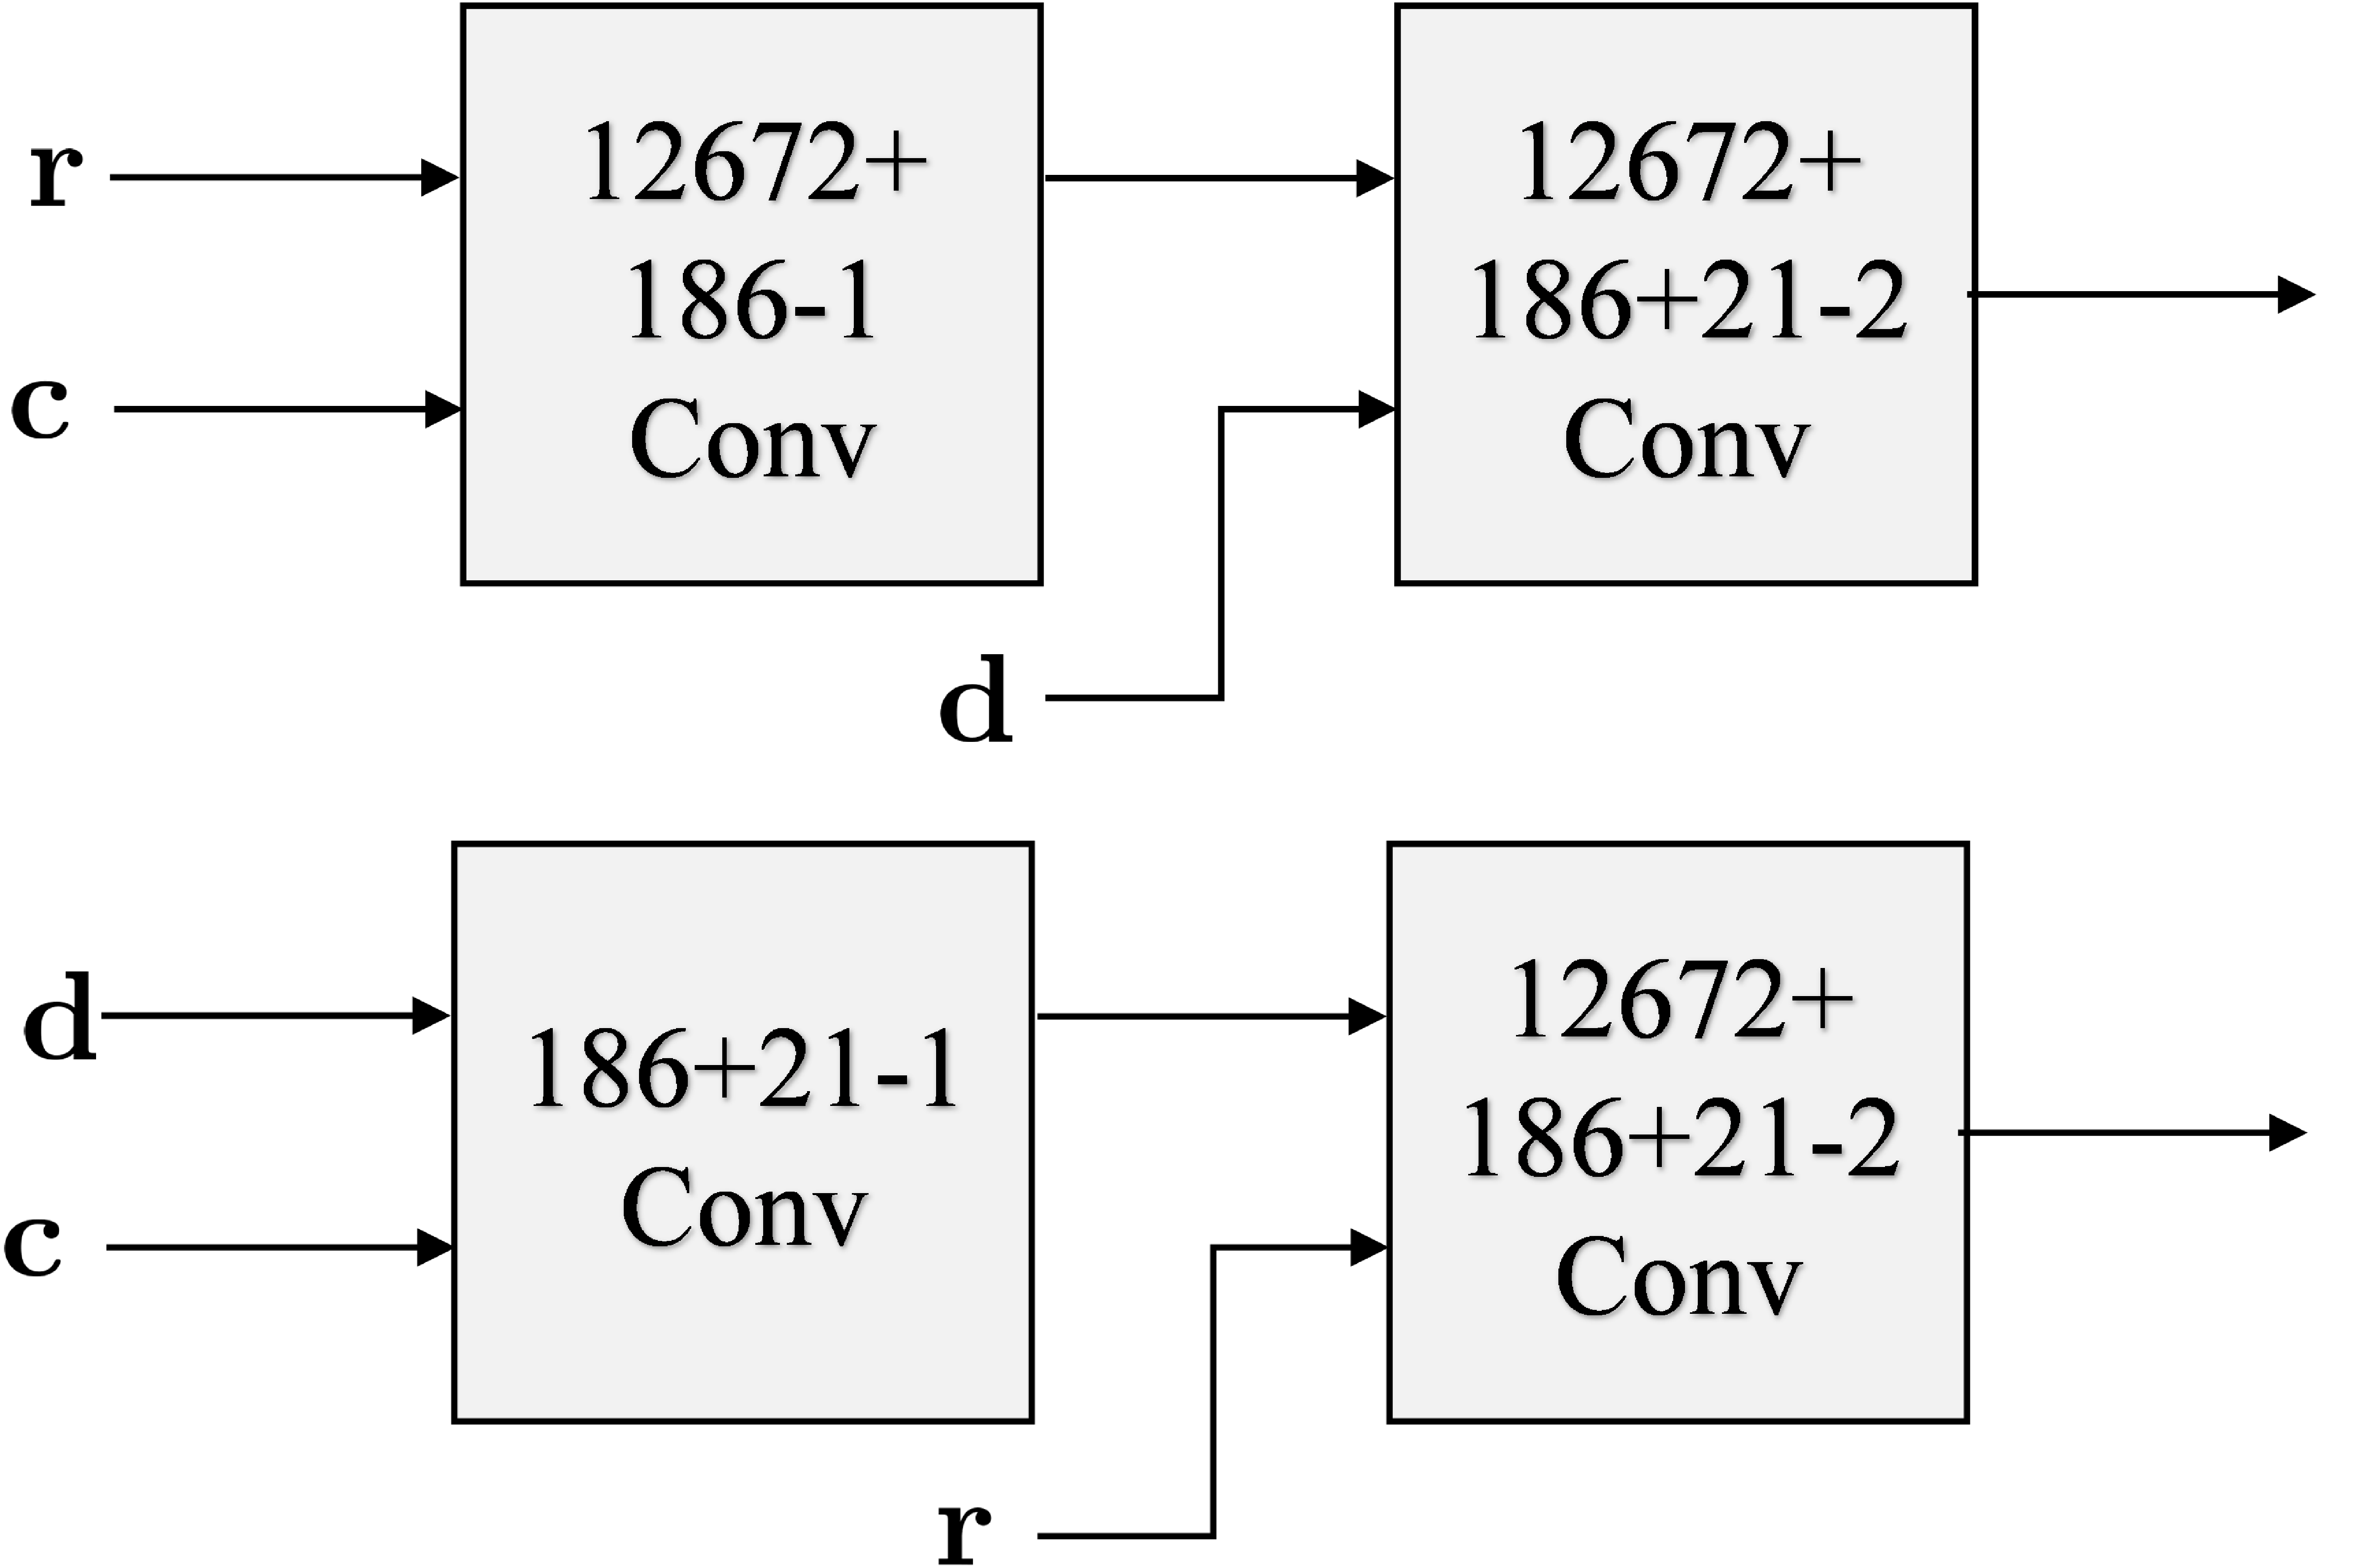
\includegraphics[width=5.01in/100*55]{figures/gpu_intro/twoWaysToConv.pdf}
	\label{fig:twoWaysToConv}
\end{figure}
Figure \ref{fig:twoWaysToConv} shows two ways to cascade the signal $\mathbf{r}$ though two filters.
The upper blocks apply both filters to the signal taking $180.272$ms then $20.4287$ms.
The lower blocks first convolve the filters to build a $186+21-1$ tap composite filter then apply the $206$ tap composite to the signal.

Table \ref{tab:Batched_CPUvsGPUtable_12672_21_186} shows the execution time of implementing cascaded filters, convolving the $21$ and $186$ tap filters is extremely fast in the GPU.
While building the composite filter is extremely fast, time domain convolution suffers a $22.0170$ms or $19.7460$ms slow down because the composite filter is now $206$ taps.
Applying an extra filter in the frequency domain only costs $2.3165$ms.
Table \ref{tab:Batched_CPUvsGPUtable_12672_206} confirms it costs an extra $20$ms or so to apply a $206$ vs $186$ tap filter.

\singlespacing
\clearpage
\begin{lstlisting}[style=myCUDAstyle,language=C++,caption={CUDA code to performing complex convolution five different ways: time domain CPU, frequency domain CPU time domain GPU, time domain GPU using shared memory and frequency domain GPU.},label={code:convFun}]
#include <iostream>
#include <stdlib.h>
#include <math.h>
#include <cufft.h>
#include <fstream>
#include <string>
#include <fftw3.h>
using namespace std;


void ConvCPU(cufftComplex* y,cufftComplex* x,cufftComplex* h,int Lx,int Lh){
	for(int yIdx = 0; yIdx < Lx+Lh-1; yIdx++){
		cufftComplex temp;
		temp.x = 0;
		temp.y = 0;
		for(int hIdx = 0; hIdx < Lh; hIdx++){
			int xAccessIdx = yIdx-hIdx;
			if(xAccessIdx>=0 && xAccessIdx<Lx){
				// temp += x[xAccessIdx]*h[hIdx];
				float A = x[xAccessIdx].x;
				float B = x[xAccessIdx].y;
				float C = h[hIdx].x;
				float D = h[hIdx].y;
				cufftComplex result;
				result.x = A*C-B*D;
				result.y = A*D+B*C;
				temp.x += result.x;
				temp.y += result.y;
			}
		}
		y[yIdx] = temp;
	}

}

__global__ void ConvGPU(cufftComplex* y,cufftComplex* x,cufftComplex* h,int Lx,int Lh){
	int yIdx = blockIdx.x*blockDim.x + threadIdx.x;

	int lastThread = Lx+Lh-1;

	// don't access elements out of bounds
	if(yIdx >= lastThread)
		return;

	cufftComplex temp;
	temp.x = 0;
	temp.y = 0;
	for(int hIdx = 0; hIdx < Lh; hIdx++){
		int xAccessIdx = yIdx-hIdx;
		if(xAccessIdx>=0 && xAccessIdx<Lx){
			// temp += x[xAccessIdx]*h[hIdx];
			float A = x[xAccessIdx].x;
			float B = x[xAccessIdx].y;
			float C = h[hIdx].x;
			float D = h[hIdx].y;
			cufftComplex result;
			result.x = A*C-B*D;
			result.y = A*D+B*C;
			temp.x += result.x;
			temp.y += result.y;
		}
	}
	y[yIdx] = temp;
}


__global__ void ConvGPUshared(cufftComplex* y,cufftComplex* x,cufftComplex* h,int Lx,int Lh){
	int yIdx = blockIdx.x*blockDim.x + threadIdx.x;

	int lastThread = Lx+Lh-1;

	extern __shared__ cufftComplex h_shared[];
	if(threadIdx.x < Lh){
		h_shared[threadIdx.x] = h[threadIdx.x];
	}
	__syncthreads();

	// don't access elements out of bounds
	if(yIdx >= lastThread)
		return;

	cufftComplex temp;
	temp.x = 0;
	temp.y = 0;
	for(int hIdx = 0; hIdx < Lh; hIdx++){
		int xAccessIdx = yIdx-hIdx;
		if(xAccessIdx>=0 && xAccessIdx<Lx){
			// temp += x[xAccessIdx]*h[hIdx];
			float A = x[xAccessIdx].x;
			float B = x[xAccessIdx].y;
			float C = h_shared[hIdx].x;
			float D = h_shared[hIdx].y;
			cufftComplex result;
			result.x = A*C-B*D;
			result.y = A*D+B*C;
			temp.x += result.x;
			temp.y += result.y;
		}
	}
	y[yIdx] = temp;
}

__global__ void PointToPointMultiply(cufftComplex* v0, cufftComplex* v1, int lastThread){
	int i = blockIdx.x*blockDim.x + threadIdx.x;

	// don't access elements out of bounds
	if(i >= lastThread)
		return;
	float A = v0[i].x;
	float B = v0[i].y;
	float C = v1[i].x;
	float D = v1[i].y;

	// (A+jB)(C+jD) = (AC-BD) + j(AD+BC)
	cufftComplex result;
	result.x = A*C-B*D;
	result.y = A*D+B*C;

	v0[i] = result;
}

__global__ void ScalarMultiply(cufftComplex* vec0, float scalar, int lastThread){
	int i = blockIdx.x*blockDim.x + threadIdx.x;

	// Don't access elements out of bounds
	if(i >= lastThread)
		return;
	cufftComplex scalarMult;
	scalarMult.x = vec0[i].x*scalar;
	scalarMult.y = vec0[i].y*scalar;
	vec0[i] = scalarMult;
}

int main(){
	int mySignalLength = 1000;
	int myFilterLength = 186;
	int myConvLength   = mySignalLength + myFilterLength - 1;
	int Nfft           = pow(2, ceil(log(myConvLength)/log(2)));

	cufftComplex *mySignal1;
	cufftComplex *mySignal2;
	cufftComplex *mySignal2_fft;

	cufftComplex *myFilter1;
	cufftComplex *myFilter2;
	cufftComplex *myFilter2_fft;

	cufftComplex *myConv1;
	cufftComplex *myConv2;
	cufftComplex *myConv2_timeReversed;
	cufftComplex *myConv3;
	cufftComplex *myConv4;
	cufftComplex *myConv5;

	mySignal1      		= (cufftComplex*)malloc(mySignalLength*sizeof(cufftComplex));
	mySignal2      		= (cufftComplex*)malloc(Nfft  		  *sizeof(cufftComplex));
	mySignal2_fft  		= (cufftComplex*)malloc(Nfft   	      *sizeof(cufftComplex));

	myFilter1      		= (cufftComplex*)malloc(myFilterLength*sizeof(cufftComplex));
	myFilter2      		= (cufftComplex*)malloc(Nfft   	      *sizeof(cufftComplex));
	myFilter2_fft  		= (cufftComplex*)malloc(Nfft  		  *sizeof(cufftComplex));

	myConv1        		= (cufftComplex*)malloc(myConvLength  *sizeof(cufftComplex));
	myConv2        		= (cufftComplex*)malloc(Nfft  	      *sizeof(cufftComplex));
	myConv2_timeReversed= (cufftComplex*)malloc(Nfft  	      *sizeof(cufftComplex));
	myConv3        		= (cufftComplex*)malloc(myConvLength  *sizeof(cufftComplex));
	myConv4        		= (cufftComplex*)malloc(myConvLength  *sizeof(cufftComplex));
	myConv5        		= (cufftComplex*)malloc(Nfft          *sizeof(cufftComplex));

	srand(time(0));
	for(int i = 0; i < mySignalLength; i++){
		mySignal1[i].x = rand()%100-50;
		mySignal1[i].y = rand()%100-50;
	}

	for(int i = 0; i < myFilterLength; i++){
		myFilter1[i].x = rand()%100-50;
		myFilter1[i].y = rand()%100-50;
	}

	cufftComplex *dev_mySignal3;
	cufftComplex *dev_mySignal4;
	cufftComplex *dev_mySignal5;

	cufftComplex *dev_myFilter3;
	cufftComplex *dev_myFilter4;
	cufftComplex *dev_myFilter5;

	cufftComplex *dev_myConv3;
	cufftComplex *dev_myConv4;
	cufftComplex *dev_myConv5;

	cudaMalloc(&dev_mySignal3, mySignalLength*sizeof(cufftComplex));
	cudaMalloc(&dev_mySignal4, mySignalLength*sizeof(cufftComplex));
	cudaMalloc(&dev_mySignal5, Nfft          *sizeof(cufftComplex));

	cudaMalloc(&dev_myFilter3, myFilterLength*sizeof(cufftComplex));
	cudaMalloc(&dev_myFilter4, myFilterLength*sizeof(cufftComplex));
	cudaMalloc(&dev_myFilter5, Nfft          *sizeof(cufftComplex));

	cudaMalloc(&dev_myConv3,   myConvLength  *sizeof(cufftComplex));
	cudaMalloc(&dev_myConv4,   myConvLength  *sizeof(cufftComplex));
	cudaMalloc(&dev_myConv5,   Nfft          *sizeof(cufftComplex));


	/**
	 * Time Domain Convolution CPU
	 */
	ConvCPU(myConv1,mySignal1,myFilter1,mySignalLength,myFilterLength);

	/**
	 * Frequency Domain Convolution CPU
	 */
	fftwf_plan forwardPlanSignal = fftwf_plan_dft_1d(Nfft, (fftwf_complex*)mySignal2,    (fftwf_complex*)mySignal2_fft, 	   FFTW_FORWARD, FFTW_MEASURE);
	fftwf_plan forwardPlanFilter = fftwf_plan_dft_1d(Nfft, (fftwf_complex*)myFilter2, 	 (fftwf_complex*)myFilter2_fft, 	   FFTW_FORWARD, FFTW_MEASURE);
	fftwf_plan backwardPlanConv  = fftwf_plan_dft_1d(Nfft, (fftwf_complex*)mySignal2_fft,(fftwf_complex*)myConv2_timeReversed, FFTW_FORWARD, FFTW_MEASURE);

	cufftComplex zero; zero.x = 0; zero.y = 0;
	for(int i = 0; i < Nfft; i++){
		if(i<mySignalLength)
			mySignal2[i] = mySignal1[i];
		else
			mySignal2[i] = zero;

		if(i<myFilterLength)
			myFilter2[i] = myFilter1[i];
		else
			myFilter2[i] = zero;
	}

	fftwf_execute(forwardPlanSignal);
	fftwf_execute(forwardPlanFilter);

	for (int i = 0; i < Nfft; i++){
		// mySignal2_fft = mySignal2_fft*myFilter2_fft;
		float A = mySignal2_fft[i].x;
		float B = mySignal2_fft[i].y;
		float C = myFilter2_fft[i].x;
		float D = myFilter2_fft[i].y;
		cufftComplex result;
		result.x = A*C-B*D;
		result.y = A*D+B*C;
		mySignal2_fft[i] = result;
	}

	fftwf_execute(backwardPlanConv);

	// myConv2 from fftwf must be time reversed and scaled
	// to match Matlab, myConv1, myConv3, myConv4 and myConv5
	cufftComplex result;
	for (int i = 0; i < Nfft; i++){
		result.x = myConv2_timeReversed[Nfft-i].x/Nfft;
		result.y = myConv2_timeReversed[Nfft-i].y/Nfft;
		myConv2[i] = result;
	}
	result.x = myConv2_timeReversed[0].x/Nfft;
	result.y = myConv2_timeReversed[0].y/Nfft;
	myConv2[0] = result;

	fftwf_destroy_plan(forwardPlanSignal);
	fftwf_destroy_plan(forwardPlanFilter);
	fftwf_destroy_plan(backwardPlanConv);


	/**
	 * Time Domain Convolution GPU Using Global Memory
	 */
	cudaMemcpy(dev_mySignal3, mySignal1, sizeof(cufftComplex)*mySignalLength, cudaMemcpyHostToDevice);
	cudaMemcpy(dev_myFilter3, myFilter1, sizeof(cufftComplex)*myFilterLength, cudaMemcpyHostToDevice);

	int numTreadsPerBlock = 512;
	int numBlocks = myConvLength/numTreadsPerBlock;
	if(myConvLength % numTreadsPerBlock > 0)
		numBlocks++;
	ConvGPU<<<numBlocks, numTreadsPerBlock>>>(dev_myConv3, dev_mySignal3, dev_myFilter3, mySignalLength, myFilterLength);

	cudaMemcpy(myConv3, dev_myConv3, myConvLength*sizeof(cufftComplex), cudaMemcpyDeviceToHost);


	/**
	 * Time Domain Convolution GPU Using Shared Memory
	 */
	cudaMemcpy(dev_mySignal4, mySignal1, sizeof(cufftComplex)*mySignalLength, cudaMemcpyHostToDevice);
	cudaMemcpy(dev_myFilter4, myFilter1, sizeof(cufftComplex)*myFilterLength, cudaMemcpyHostToDevice);

	numTreadsPerBlock = 512;
	numBlocks = myConvLength/numTreadsPerBlock;
	if(myConvLength % numTreadsPerBlock > 0)
		numBlocks++;
	ConvGPUshared<<<numBlocks, numTreadsPerBlock,myFilterLength*sizeof(cufftComplex)>>>(dev_myConv4, dev_mySignal4, dev_myFilter4, mySignalLength, myFilterLength);

	cudaMemcpy(myConv4, dev_myConv4, myConvLength*sizeof(cufftComplex), cudaMemcpyDeviceToHost);


	/**
	 * Frequency Domain Convolution GPU
	 */
	cufftHandle plan;
	int n[1] = {Nfft};
	cufftPlanMany(&plan,1,n,NULL,1,1,NULL,1,1,CUFFT_C2C,1);

	cudaMemset(dev_mySignal5, 0, 	     Nfft*sizeof(cufftComplex));
	cudaMemset(dev_myFilter5, 0, 	     Nfft*sizeof(cufftComplex));

	cudaMemcpy(dev_mySignal5, mySignal2, Nfft*sizeof(cufftComplex), cudaMemcpyHostToDevice);
	cudaMemcpy(dev_myFilter5, myFilter2, Nfft*sizeof(cufftComplex), cudaMemcpyHostToDevice);

	cufftExecC2C(plan, dev_mySignal5, dev_mySignal5, CUFFT_FORWARD);
	cufftExecC2C(plan, dev_myFilter5, dev_myFilter5, CUFFT_FORWARD);

	numTreadsPerBlock = 512;
	numBlocks = Nfft/numTreadsPerBlock;
	if(Nfft % numTreadsPerBlock > 0)
		numBlocks++;
	PointToPointMultiply<<<numBlocks, numTreadsPerBlock>>>(dev_mySignal5, dev_myFilter5, Nfft);

	cufftExecC2C(plan, dev_mySignal5, dev_mySignal5, CUFFT_INVERSE);

	numTreadsPerBlock = 128;
	numBlocks = Nfft/numTreadsPerBlock;
	if(Nfft % numTreadsPerBlock > 0)
		numBlocks++;
	float scalar = 1.0/((float)Nfft);
	ScalarMultiply<<<numBlocks, numTreadsPerBlock>>>(dev_mySignal5, scalar, Nfft);

	cudaMemcpy(myConv5, dev_mySignal5, Nfft*sizeof(cufftComplex), cudaMemcpyDeviceToHost);

	cufftDestroy(plan);

	free(mySignal1);
	free(mySignal2);

	free(myFilter1);
	free(myFilter2);

	free(myConv1);
	free(myConv2);
	free(myConv2_timeReversed);
	free(myConv3);
	free(myConv4);
	free(myConv5);
	fftwf_cleanup();

	cudaFree(dev_mySignal3);
	cudaFree(dev_mySignal4);
	cudaFree(dev_mySignal5);

	cudaFree(dev_myFilter3);
	cudaFree(dev_myFilter4);
	cudaFree(dev_myFilter5);

	cudaFree(dev_myConv3);
	cudaFree(dev_myConv4);
	cudaFree(dev_myConv5);

	return 0;
}
\end{lstlisting}
\doublespacing

\singlespacing
\clearpage
\begin{lstlisting}[style=myCUDAstyle,language=C++,caption={CUDA code to perform batched complex convolution three different ways in a GPU: time domain using global memory, time domain using shared memory and frequency domain GPU.},label={code:batchedConvFun}]
#include <cufft.h>
#include <iostream>
using namespace std;

__global__ void ConvGPU(cufftComplex* y_out,cufftComplex* x_in,cufftComplex* h_in,int Lx,int Lh,int maxThreads){
	int threadNum = blockIdx.x*blockDim.x + threadIdx.x;
	int convLength = Lx+Lh-1;

	// Don't access elements out of bounds
	if(threadNum >= maxThreads)
		return;

	int batch = threadNum/convLength;
	int yIdx  = threadNum%convLength;
	cufftComplex* x = &x_in[Lx*batch];
	cufftComplex* h = &h_in[Lh*batch];
	cufftComplex* y = &y_out[convLength*batch];

	cufftComplex temp;
	temp.x = 0;
	temp.y = 0;
	for(int hIdx = 0; hIdx < Lh; hIdx++){
		int xAccessIdx = yIdx-hIdx;
		if(xAccessIdx>=0 && xAccessIdx<Lx){
			// temp += x[xAccessIdx]*h[hIdx];
			// (A+jB)(C+jD) = (AC-BD) + j(AD+BC)
			float A = x[xAccessIdx].x;
			float B = x[xAccessIdx].y;
			float C = h[hIdx].x;
			float D = h[hIdx].y;
			cufftComplex complexMult;
			complexMult.x = A*C-B*D;
			complexMult.y = A*D+B*C;

			temp.x += complexMult.x;
			temp.y += complexMult.y;
		}
	}
	y[yIdx] = temp;
}

__global__ void ConvGPUshared(cufftComplex* y_out,cufftComplex* x_in,cufftComplex* h_in,int Lx,int Lh,int maxThreads){

	int threadNum = blockIdx.x*blockDim.x + threadIdx.x;
	int convLength = Lx+Lh-1;
	// Don't access elements out of bounds
	if(threadNum >= maxThreads)
		return;

	int batch = threadNum/convLength;
	int yIdx  = threadNum%convLength;
	cufftComplex* x = &x_in[Lx*batch];
	cufftComplex* h = &h_in[Lh*batch];
	cufftComplex* y = &y_out[convLength*batch];

	extern __shared__ cufftComplex h_shared[];
	if(threadIdx.x < Lh)
		h_shared[threadIdx.x] = h[threadIdx.x];

	__syncthreads();

	cufftComplex temp;
	temp.x = 0;
	temp.y = 0;
	for(int hIdx = 0; hIdx < Lh; hIdx++){
		int xAccessIdx = yIdx-hIdx;
		if(xAccessIdx>=0 && xAccessIdx<Lx){
			// temp += x[xAccessIdx]*h[hIdx];
			// (A+jB)(C+jD) = (AC-BD) + j(AD+BC)
			float A = x[xAccessIdx].x;
			float B = x[xAccessIdx].y;
			float C = h_shared[hIdx].x;
			float D = h_shared[hIdx].y;
			cufftComplex complexMult;
			complexMult.x = A*C-B*D;
			complexMult.y = A*D+B*C;

			temp.x += complexMult.x;
			temp.y += complexMult.y;
		}
	}
	y[yIdx] = temp;
}

__global__ void PointToPointMultiply(cufftComplex* vec0, cufftComplex* vec1, int maxThreads){
	int i = blockIdx.x*blockDim.x + threadIdx.x;
	// Don't access elements out of bounds
	if(i >= maxThreads)
		return;
	// vec0[i] = vec0[i]*vec1[i];
	// (A+jB)(C+jD) = (AC-BD) + j(AD+BC)
	float A = vec0[i].x;
	float B = vec0[i].y;
	float C = vec1[i].x;
	float D = vec1[i].y;
	cufftComplex complexMult;
	complexMult.x = A*C-B*D;
	complexMult.y = A*D+B*C;
	vec0[i] = complexMult;
}

__global__ void ScalarMultiply(cufftComplex* vec0, float scalar, int lastThread){
	int i = blockIdx.x*blockDim.x + threadIdx.x;
	// Don't access elements out of bounds
	if(i >= lastThread)
		return;
	cufftComplex scalarMult;
	scalarMult.x = vec0[i].x*scalar;
	scalarMult.y = vec0[i].y*scalar;
	vec0[i] = scalarMult;
}

int main(){
	int numBatches     = 3104;
	int mySignalLength = 12672;
	int myFilterLength = 186;
	int myConvLength   = mySignalLength + myFilterLength - 1;
	int Nfft           = pow(2, ceil(log(myConvLength)/log(2)));
	int maxThreads;
	int numTreadsPerBlock;
	int numBlocks;

	cufftHandle plan;
	int n[1] = {Nfft};
	cufftPlanMany(&plan,1,n,NULL,1,1,NULL,1,1,CUFFT_C2C,numBatches);

	// Allocate memory on host
	cufftComplex *mySignal1;
	cufftComplex *mySignal1_pad;
	cufftComplex *myFilter1;
	cufftComplex *myFilter1_pad;
	cufftComplex *myConv1;
	cufftComplex *myConv2;
	cufftComplex *myConv3;
	mySignal1      = (cufftComplex*) malloc(mySignalLength*numBatches*sizeof(cufftComplex));
	mySignal1_pad  = (cufftComplex*) malloc(Nfft		  *numBatches*sizeof(cufftComplex));
	myFilter1      = (cufftComplex*) malloc(myFilterLength*numBatches*sizeof(cufftComplex));
	myFilter1_pad  = (cufftComplex*) malloc(Nfft	      *numBatches*sizeof(cufftComplex));
	myConv1        = (cufftComplex*) malloc(myConvLength  *numBatches*sizeof(cufftComplex));
	myConv2        = (cufftComplex*) malloc(myConvLength  *numBatches*sizeof(cufftComplex));
	myConv3        = (cufftComplex*) malloc(Nfft		  *numBatches*sizeof(cufftComplex));

	srand(time(0));
	for(int i = 0; i < mySignalLength; i++){
		mySignal1[i].x = rand()%100-50;
		mySignal1[i].y = rand()%100-50;
	}

	for(int i = 0; i < myFilterLength; i++){
		myFilter1[i].x = rand()%100-50;
		myFilter1[i].y = rand()%100-50;
	}

	cufftComplex zero;
	zero.x = 0;
	zero.y = 0;
	for(int i = 0; i<Nfft*numBatches; i++){
		mySignal1_pad[i] = zero;
		myFilter1_pad[i] = zero;
	}
	for(int batch=0; batch < numBatches; batch++){
		for(int i = 0; i < mySignalLength; i++){
			mySignal1[batch*mySignalLength+i] = mySignal1[i];
			mySignal1_pad[batch*Nfft+i] = mySignal1[i];
		}
		for(int i = 0; i < myFilterLength; i++){
			myFilter1[batch*myFilterLength+i] = myFilter1[i];
			myFilter1_pad[batch*Nfft+i] = myFilter1[i];
		}
	}

	// Allocate memory on device
	cufftComplex *dev_mySignal1;
	cufftComplex *dev_mySignal2;
	cufftComplex *dev_mySignal3;
	cufftComplex *dev_myFilter1;
	cufftComplex *dev_myFilter2;
	cufftComplex *dev_myFilter3;
	cufftComplex *dev_myConv1;
	cufftComplex *dev_myConv2;
	cufftComplex *dev_myConv3;
	cudaMalloc(&dev_mySignal1, mySignalLength*numBatches*sizeof(cufftComplex));
	cudaMalloc(&dev_mySignal2, mySignalLength*numBatches*sizeof(cufftComplex));
	cudaMalloc(&dev_mySignal3, Nfft		     *numBatches*sizeof(cufftComplex));
	cudaMalloc(&dev_myFilter1, myFilterLength*numBatches*sizeof(cufftComplex));
	cudaMalloc(&dev_myFilter2, myFilterLength*numBatches*sizeof(cufftComplex));
	cudaMalloc(&dev_myFilter3, Nfft			 *numBatches*sizeof(cufftComplex));
	cudaMalloc(&dev_myConv1,   myConvLength  *numBatches*sizeof(cufftComplex));
	cudaMalloc(&dev_myConv2,   myConvLength  *numBatches*sizeof(cufftComplex));
	cudaMalloc(&dev_myConv3,   Nfft  		 *numBatches*sizeof(cufftComplex));

	/**
	 * Time Domain Convolution GPU Using Global Memory
	 */
	cudaMemcpy(dev_mySignal1, mySignal1, numBatches*sizeof(cufftComplex)*mySignalLength, cudaMemcpyHostToDevice);
	cudaMemcpy(dev_myFilter1, myFilter1, numBatches*sizeof(cufftComplex)*myFilterLength, cudaMemcpyHostToDevice);

	maxThreads = myConvLength*numBatches;
	numTreadsPerBlock = 128;
	numBlocks = maxThreads/numTreadsPerBlock;
	if(maxThreads % numTreadsPerBlock > 0)
		numBlocks++;
	ConvGPU<<<numBlocks, numTreadsPerBlock>>>(dev_myConv1, dev_mySignal1, dev_myFilter1, mySignalLength, myFilterLength, maxThreads);

	cudaMemcpy(myConv1, dev_myConv1, myConvLength*numBatches*sizeof(cufftComplex), cudaMemcpyDeviceToHost);

	/**
	 * Time Domain Convolution GPU Using Shared Memory
	 */
	cudaMemcpy(dev_mySignal2, mySignal1, numBatches*sizeof(cufftComplex)*mySignalLength, cudaMemcpyHostToDevice);
	cudaMemcpy(dev_myFilter2, myFilter1, numBatches*sizeof(cufftComplex)*myFilterLength, cudaMemcpyHostToDevice);

	maxThreads = myConvLength*numBatches;
	numTreadsPerBlock = 256;
	numBlocks = maxThreads/numTreadsPerBlock;
	if(maxThreads % numTreadsPerBlock > 0)
		numBlocks++;
	ConvGPUshared<<<numBlocks, numTreadsPerBlock, myFilterLength*sizeof(cufftComplex)>>>(dev_myConv2, dev_mySignal2, dev_myFilter2, mySignalLength, myFilterLength,maxThreads);

	cudaMemcpy(myConv2, dev_myConv2, myConvLength*numBatches*sizeof(cufftComplex), cudaMemcpyDeviceToHost);

	/**
	 * Frequency Domain Convolution GPU
	 */
	cudaMemcpy(dev_mySignal3, mySignal1_pad, Nfft*numBatches*sizeof(cufftComplex), cudaMemcpyHostToDevice);
	cudaMemcpy(dev_myFilter3, myFilter1_pad, Nfft*numBatches*sizeof(cufftComplex), cudaMemcpyHostToDevice);

	cufftExecC2C(plan, dev_mySignal3, dev_mySignal3, CUFFT_FORWARD);
	cufftExecC2C(plan, dev_myFilter3, dev_myFilter3, CUFFT_FORWARD);

	maxThreads = Nfft*numBatches;
	numTreadsPerBlock = 96;
	numBlocks = maxThreads/numTreadsPerBlock;
	if(maxThreads % numTreadsPerBlock > 0)
		numBlocks++;
	PointToPointMultiply<<<numBlocks, numTreadsPerBlock>>>(dev_mySignal3, dev_myFilter3, maxThreads);
	cufftExecC2C(plan, dev_mySignal3, dev_mySignal3, CUFFT_INVERSE);

	numTreadsPerBlock = 640;
	numBlocks = maxThreads/numTreadsPerBlock;
	if(maxThreads % numTreadsPerBlock > 0)
		numBlocks++;
	float scalar = 1.0/((float)Nfft);
	ScalarMultiply<<<numBlocks, numTreadsPerBlock>>>(dev_mySignal3, scalar, maxThreads);

	cudaMemcpy(myConv3, dev_mySignal3, Nfft*numBatches*sizeof(cufftComplex), cudaMemcpyDeviceToHost);

	cufftDestroy(plan);

	// Free vectors on CPU
	free(mySignal1);
	free(myFilter1);
	free(myConv1);
	free(myConv2);
	free(myConv3);

	// Free vectors on GPU
	cudaFree(dev_mySignal1);
	cudaFree(dev_mySignal2);
	cudaFree(dev_mySignal3);
	cudaFree(dev_myFilter1);
	cudaFree(dev_myFilter2);
	cudaFree(dev_myFilter3);
	cudaFree(dev_myConv1);
	cudaFree(dev_myConv2);
	cudaFree(dev_myConv3);

	return 0;
}
\end{lstlisting}
\doublespacing